% SI.tex – Supplementary Information for
% "AMOC projections are uncertain because they depend on model and reanalysis choice"
% Compile: pdflatex SI.tex && bibtex SI && pdflatex SI.tex

\documentclass[10pt,a4paper]{article}
\usepackage[utf8]{inputenc}
\usepackage[T1]{fontenc}
\usepackage[margin=2.5cm]{geometry}
\usepackage{graphicx}
\usepackage{subcaption}
\usepackage{amsmath,amssymb}
\usepackage{natbib}
\usepackage{lineno}
\usepackage{booktabs}

% Custom commands
\newcommand{\Fovs}{F_{\mathrm{ovS}}}
\newcommand{\dFv}{\Delta F_v}
\newcommand{\dFs}{\Delta F_s}
\newcommand{\dFc}{\Delta F_{\mathrm{cross}}}

\title{Supplementary Information  \\
}
%\author{B. Fallah, L.-Y. Fu, J. Guo, M. Rostami}
\date{}

\graphicspath{{../figures/paper2/}}

\begin{document}
\maketitle

\section*{Methods}
\linenumbers

\subsection*{Observational reanalysis datasets}

Four independent global ocean reanalysis products are analysed. They were selected to span the four mainstream data-assimilation paradigms in the global-ocean reanalysis ecosystem -- 3D-Var FGAT (ORAS5), reduced-order Kalman filter with 3D-Var bias correction (GLORYS12V1), ensemble optimal interpolation (SODA 3.15.2), and 4D-variational adjoint state estimation (ECCO-V4r4) -- and together cover the eddy-resolving ($1/12^\circ$) to coarse-resolution ($1/2^\circ$) range used in CMIP-class climate analysis. This is the same four-product canonical ensemble adopted by the headline emergent-constraint study \citep{Portmann2026}, ensuring that our mechanism decomposition is directly comparable to that constraint without product-selection ambiguity. Adding a fifth product from any of the same paradigms (e.g.~ORAS4, C-GLORS, FOAM) would not break the velocity-vs-salinity dichotomy because such siblings share systematic biases with their corresponding family member; a complementary GECCO3 (Hamburg) 4D-Var run would be the most informative future addition because it would test whether the ECCO null trend is generic to adjoint optimisation. The four products together represent the currently available space of observationally-constrained three-dimensional ocean state estimates at 34.5$^\circ$S.

\paragraph{ORAS5} \citep{Zuo2019}. Ocean Reanalysis System 5 from ECMWF. Native grid: ORCA025 tripolar (nominal $\sim$1/4$^\circ$, $\sim$25~km at the equator and $\sim$14~km at 34.5$^\circ$S after the $\cos\phi$ contraction), 75 vertical levels with 1-m surface resolution. NEMOVAR 3D-Var FGAT data-assimilation scheme ingesting sub-surface temperature/salinity profiles, sea-ice concentration, and along-track altimetric sea-level anomalies. Atmospheric forcing: ERA-40 (1958--1978) transitioning to ERA-Interim/ERA5 (1979--present). Record used: 816 monthly means, 1958--2025.

\paragraph{GLORYS12V1} \citep{Lellouche2021}. Copernicus Marine Service/Mercator Ocean global ocean reanalysis at 1/12$^\circ$ ($\sim$8~km, eddy-resolving), 50 vertical levels. A reduced-order Kalman filter (SAM2) jointly assimilates along-track altimetry, satellite sea-surface temperature, sea-ice concentration, and in-situ CTD and Argo temperature/salinity profiles, supplemented by 3D-Var bias correction. Atmospheric forcing: ERA5. Record used: 396 monthly means, 1993--2025 (satellite-altimetry era).

\paragraph{SODA 3.15.2} \citep{Carton2018}. Simple Ocean Data Assimilation 3 from the University of Maryland. Native grid: MOM5 $\sim$1/2$^\circ$ (regridded to a uniform 0.5$^\circ$ product on the UMD mirror), 50 vertical levels. Assimilation scheme: ensemble optimal interpolation with a 5-day analysis cycle; the downloadable output is a sequence of 5-day snapshots. Atmospheric forcing: MERRA-2. We sample four 5-day snapshots per year (mid-month of January, April, July, October) to approximate the annual mean, consistent with previous applications of the same product to overturning-transport diagnostics. Record used: 43 annual means, 1980--2022.

\paragraph{ECCO-V4r4} \citep{Forget2015}. NASA/JPL Estimating the Circulation and Climate of the Ocean, version 4 release 4. Native grid: LLC90 Lat-Lon-Cap (regridded to a uniform 0.5$^\circ$ monthly product), 50 vertical levels. ECCO is an adjoint-based least-squares state estimate (4D-variational) that iteratively adjusts initial conditions, surface fluxes, and interior mixing to minimise the misfit between the model trajectory and the full suite of altimetry, Argo, satellite SST/SSH, and mooring observations over its full time span. Atmospheric forcing (post-iteration): an ECCO-adjusted ERA-family atmospheric analysis. Record used: 26 annual means, 1992--2017.

\paragraph{Direct-hydrography anchors.} Three published overturning freshwater-transport estimates at 34.5$^\circ$S from direct in-situ observations are used as independent anchor points in Fig.~1: \citet{GarzoliMatano2011} (central year 2005, value $-0.10\pm0.10$~Sv); \citet{Meinen2018} (central year 2015, value $-0.09\pm0.05$~Sv); and \citet{Kersale2020} (central year 2015, value $-0.17\pm0.07$~Sv). Together with \citet{Dong2024}'s $-0.15\pm0.09$~Sv from 49 XBT transects, they bracket the reanalysis ensemble from the low side.

\subsection*{CMIP6 ensemble}

CMIP6 meridional-velocity (\texttt{vo}) and salinity (\texttt{so}) sections at 34.5$^\circ$S are obtained for every available model with coverage of both the \texttt{historical} experiment (required period 1950--1980) and the \texttt{ssp585} experiment (required period 2080--2100). The native grid of each model is used (i.e. no regridding), because regridding distorts the mechanistic decomposition. Fifteen models satisfy both criteria with accessible section files: CESM2, CMCC-CM2-SR5, CNRM-CM6-1, CanESM5, FGOALS-g3, FIO-ESM-2-0, GFDL-CM4, GISS-E2-1-G, HadGEM3-GC31-LL, IPSL-CM6A-LR, MIROC6, MPI-ESM1-2-HR, MPI-ESM1-2-LR, NESM3, UKESM1-0-LL. Three models are excluded: NorESM2-LM and NorESM2-MM because their ocean component is on isopycnal (density) coordinates and cannot be integrated in depth-space without an additional remap that would confound the decomposition; and ACCESS-CM2 because its accessible \texttt{ssp585} run does not extend to 2100. All models use the \texttt{r1i1p1f1} realisation.

A 13-model subset with \texttt{piControl} access is used for the internal-variability null test: ACCESS-CM2, CESM2, CMCC-CM2-SR5, CNRM-CM6-1, CanESM5, GISS-E2-1-G, HadGEM3-GC31-LL, IPSL-CM6A-LR, MIROC6, MPI-ESM1-2-HR, MPI-ESM1-2-LR, NESM3, UKESM1-0-LL.

\paragraph{Ensemble size used per analysis.} Different downstream analyses retain different subsets of the 15-model decomposition ensemble:

\begin{itemize}
\item \emph{Mechanism decomposition + tiebreaker scatter} (Figs.~1b, 2a of the main text): all 15 models. Three models are flagged \emph{increasing} (CMCC-CM2-SR5, CanESM5, IPSL-CM6A-LR) and excluded from the mechanism-conditional projection because their forced $\Fovs$ change is positive; this leaves \textbf{12 weakening models} that drive the headline 10-percentage-point gap (Figs.~2b,~2c).
\item \emph{Bistable-only subset} (Fig.~3): 6 models have $\overline{\Fovs}(t_1)<0$; of those, 2 are \emph{increasing} and are dropped, leaving \textbf{$n=4$ weakening + bistable} models (CNRM-CM6-1, MIROC6 salinity-dominant; MPI-ESM1-2-HR, NESM3 velocity-dominant).
\item \emph{piControl null} (Fig.~4c): \textbf{13 models} (the subset listed above), with up to 200 random non-overlapping 30-year window pairs per model.
\item \emph{Lead-lag cross-correlation} (Fig.~6a) and \emph{emergent constraint regression} (Fig.~6b): \textbf{16 models}. Both diagnostics use only the 1850-2024 historical+\texttt{ssp585} window for the lead-lag and the 2000-2024 / 2030-2040 windows for the emergent constraint, which means ACCESS-CM2 -- excluded from the decomposition because its \texttt{ssp585} run does not reach 2100 -- can be retained here. We re-add it to maximise statistical power on the lead-lag cross-correlation function and on the regression slope.
\end{itemize}

This per-analysis bookkeeping is reflected in each figure's panel-internal $n=$ labels and in the captions of the main text.

\subsection*{Section extraction and grid metrics}

At each time step of each product we extract the zonal-depth section at the gridded latitude closest to $-34.5^\circ$. Where the ocean-model grid is staggered (e.g. velocity at U-points and salinity at T-points on the ORAS5 NEMO grid), the two fields are extracted on their native grids and aligned by truncation to the common Atlantic-longitude mask.

The Atlantic basin at 34.5$^\circ$S is defined by the longitude range $[-70^\circ, 20^\circ]$ in the $[-180^\circ, 180^\circ]$ convention (bounds chosen inclusively to cover from the Argentine coast to the African coast while excluding residual Agulhas leakage; the small $<1\%$ contribution from the strictly-classified Drake-Passage edge does not alter the results).

The zonal grid spacing at each Atlantic U-point is
\[
\Delta x_i = |\Delta\lambda_i|\, R_\oplus\, \cos\phi,
\]
with $\Delta\lambda_i$ the local longitudinal grid spacing (after longitude wrap-around correction), $R_\oplus = 111$~km per degree at the equator, and $\phi = -34.5^\circ$. Vertical cell thicknesses $\Delta z_k$ are taken directly from the product's vertical coordinate (with the CESM-family POP grid converted from centimetres to metres).

\subsection*{$\Fovs$ computation}

We follow the definition of \citet{deVriesWeber2005}, used also by \citet{Dijkstra2007, Drijfhout2011, vanWesten2024}:
\[
\Fovs = -\frac{1}{S_0}\int_{z_\mathrm{bot}}^{z_\mathrm{surf}}
  V_\mathrm{int}(z)\,[\bar{S}(z) - S_0]\,\mathrm{d}z,
\]
with
\[
V_\mathrm{int}(z) = \sum_{i\in\mathrm{Atl}} v(x_i, z)\,\Delta x_i \qquad(\mathrm{m}^2/\mathrm{s}),
\]
and
\[
\bar{S}(z) = \frac{\sum_{i\in\mathrm{Atl}} S(x_i, z)\,\Delta x_i
                  \cdot m(x_i, z)}
                 {\sum_{i\in\mathrm{Atl}} \Delta x_i \cdot m(x_i, z)},
\]
where $m(x_i, z)\in\{0, 1\}$ is the wet-cell mask (unity over the ocean, zero over bathymetry). The reference salinity is fixed at $S_0 = 35$~PSU throughout. The integral is evaluated by a discrete sum over vertical levels using the native $\Delta z_k$ as quadrature weights; the final result is reported in Sverdrups (Sv = $10^6~\mathrm{m}^3/\mathrm{s}$). This kernel is implemented once in \texttt{ardp/physics/fovs.py} and reused for every product (reanalyses, CMIP6 historical/ssp585, piControl) to eliminate cross-product inconsistencies.

\subsubsection*{Barotropic-velocity subtraction}

$\Fovs$ is, by construction, the freshwater transport carried by the zonally-averaged \emph{overturning} (baroclinic) circulation, i.e. the component with $\int V_\mathrm{int}(z)\,\mathrm{d}z = 0$ across the section. In a mass-conserving model the net volume transport through a zonal section is exactly zero, so this constraint is satisfied automatically. Data-assimilating Boussinesq reanalyses (ORAS5, GLORYS12V1, SODA~3.15.2, ECCO-V4r4) and Boussinesq coupled models in CMIP6, however, do \emph{not} enforce volume conservation across an arbitrary zonal section, and their net transport $V_\mathrm{net} = \int V_\mathrm{int}(z)\,\mathrm{d}z$ generally takes non-zero values that drift slowly between months and decades as data-assimilation increments or parameterised surface sources re-balance the basin. If this drift is left in, it couples to the offset $\bar{S}(z) - S_0$ and injects a spurious mSv-scale signal into $\Fovs$ that has nothing to do with the overturning.

We therefore follow \citet{deVriesWeber2005, Mecking2017, Weijer2019} and explicitly subtract the section-mean (barotropic) velocity
\[
\bar{v}_\mathrm{bt} \equiv
   \frac{\int V_\mathrm{int}(z)\,\mathrm{d}z}
        {\int A_{xy}(z)\,\mathrm{d}z},
  \qquad
A_{xy}(z) \equiv \sum_{i\in\mathrm{Atl}} \Delta x_i\,m(x_i, z),
\]
before evaluating $\Fovs$, replacing $V_\mathrm{int}(z)$ by its baroclinic residual $V_\mathrm{int}^{\mathrm{bc}}(z) \equiv V_\mathrm{int}(z) - \bar{v}_\mathrm{bt}\,A_{xy}(z)$. By construction, $\int V_\mathrm{int}^{\mathrm{bc}}(z)\,\mathrm{d}z \equiv 0$, which eliminates the volume-drift artefact. The subtraction is applied independently to each monthly snapshot of each product (so the correction tracks the DA increments in time) and is enforced identically on all four reanalyses, on all CMIP6 models, and on the \texttt{piControl} null ensemble.

Across the two decomposition windows reported here the magnitude of $V_\mathrm{net}$ is $\sim0.9$--$1.4$~Sv for ORAS5 and GLORYS12V1, $\sim1.1$--$1.3$~Sv for ECCO-V4r4, and $\sim3.8$--$5.0$~Sv for SODA 3.15.2 (see Table~1 in main text); the $\sim10$--$40$~mSv spurious contribution that the correction removes is therefore of the same order as the $|\Delta\Fovs|$ signals that drive the mechanism classification, and its omission would have qualitatively flipped the classification in several cases. An independent unit test in \texttt{tests/test\_fovs\_decomposition.py} verifies the $\Delta\Fovs = 0$ identity for a pure uniform-velocity drift between two periods.

\subsection*{Mechanism decomposition}

Define $\Delta\Fovs \equiv \Fovs(t_2) - \Fovs(t_1)$ for two non-overlapping period averages $t_1$ (``early'') and $t_2$ (``late''). Writing $v_2 \equiv v_1 + \Delta v$ and $\bar{S}_2 \equiv \bar{S}_1 + \Delta\bar{S}$ and substituting into the definition of $\Fovs$ gives the exact identity
\[
\Delta \Fovs = \dFv + \dFs + \dFc,
\]
where
\[
\begin{aligned}
\dFv &= -\frac{1}{S_0}\int \Delta V_\mathrm{int}(z)\,
        [\bar{S}_1(z) - S_0]\,\mathrm{d}z,\\[2pt]
\dFs &= -\frac{1}{S_0}\int V_{\mathrm{int},1}(z)\,
        \Delta\bar{S}(z)\,\mathrm{d}z,\\[2pt]
\dFc &= -\frac{1}{S_0}\int \Delta V_\mathrm{int}(z)\,
        \Delta\bar{S}(z)\,\mathrm{d}z.
\end{aligned}
\]
$\dFv$ is the change that would have occurred if only the velocity field had changed (salinity frozen at its $t_1$ value); $\dFs$ is the change that would have occurred if only the zonal-mean salinity had changed (velocity frozen at $t_1$); and $\dFc$ is the cross (``eddy'') term that is zero when $\Delta v$ and $\Delta\bar{S}$ are exactly orthogonal in a depth-integrated sense and becomes large and signed when the two anomalies are correlated in $z$. The identity is exact up to floating-point round-off; unit tests verify residual magnitudes of $\mathcal{O}(10^{-15})$~Sv across randomised synthetic sections, velocity-only perturbations, salinity-only perturbations, and land-masked cases.

The \emph{velocity share} and \emph{salinity share} reported throughout are
\[
f_v \equiv 100\cdot \dFv/\Delta\Fovs,\qquad
f_s \equiv 100\cdot \dFs/\Delta\Fovs,\qquad
f_c \equiv 100\cdot \dFc/\Delta\Fovs,
\]
with the exact constraint $f_v + f_s + f_c = 100\%$. An individual share can exceed $100\%$ or be negative whenever the three components do not all carry the same sign. This occurs naturally in the salt-advection-feedback regime when $\Delta v$ and $\Delta\bar{S}$ are anti-correlated in the vertical (e.g. a slowed upper-limb circulation combined with a freshened subtropical layer); then $\dFc$ becomes large and of opposite sign to $\dFv + \dFs$, so that $|f_v|$ and $|f_s|$ each exceed $100\%$. Values $|f_v| > 100\%$ therefore indicate a physically meaningful cross-term, not a numerical artefact.

The decomposition becomes numerically ill-conditioned when $|\Delta\Fovs|$ is small relative to $|\dFv|$, $|\dFs|$, or $|\dFc|$. We pre‑registered a threshold of $|\Delta\Fovs| \ge 10$~mSv below which the mechanism decomposition is declared \emph{ill-defined}. ECCO-V4r4 is the only reanalysis flagged under this rule.

\subsection*{Period choice}

The early and late periods were pre‑registered before processing the fourth reanalysis (SODA 3.15.2): $t_1 = 1993$--$2005$ and $t_2 = 2013$--$2025$. These are the longest non-overlapping windows fully within the common GLORYS12V1 record, avoiding the first few years of the satellite-altimetry era (pre‑1993) while preserving a $\gtrsim10$-year separation. For products with shorter records we use the nearest-in-length late window: SODA 3.15.2 uses $t_2 = 2013$--$2020$; ECCO-V4r4 uses $t_2 = 2013$--$2017$. For CMIP6 we pair historical 1950--1980 against \texttt{ssp585} 2080--2100 to maximise the forced signal-to-noise ratio.

The sensitivity of the classification to the period choice is reported in Fig.~4\textbf{(b)} of the main text by repeating the computation across a grid of $(t_{1,\mathrm{end}}, t_{2,\mathrm{start}})$ pairs ($t_{1,\mathrm{end}}\in\{2001,2003,2005,2007,2009\}$, $t_{2,\mathrm{start}}\in\{2011,2013,2015,2017,2019\}$, always with $t_{1,\mathrm{start}}=1993$ and $t_{2,\mathrm{end}}$ at each product's data end). The resulting 25-point distribution of $f_v$ values is reported per product.

\subsection*{Baseline regime classification}

Beyond the mechanism decomposition, each product and CMIP6 model is classified by its \emph{baseline} regime at the $t_1$ window: \emph{bistable} if $\overline{\Fovs}(t_1) < 0$ (salt-advection feedback active, \citet{Rahmstorf1996}) or \emph{monostable} if $\overline{\Fovs}(t_1) > 0$. This matters because the salt-advection feedback is not physically active in the monostable regime, so a mechanism-classification result from a monostable CMIP6 model is not directly comparable to an observational reanalysis in which the Atlantic is bistable. In our ensemble 6/15 CMIP6 models are bistable at baseline (CNRM-CM6-1, CanESM5, IPSL-CM6A-LR, MIROC6, MPI-ESM1-2-HR, NESM3); 9/15 are monostable — the well-known ``CMIP6 fresh bias'' at the South Atlantic \citep{Mecking2017, Weijer2019, Portmann2026}.

\subsection*{Trend significance}

Annual-mean $\Fovs$ time series are analysed for linear trends under three complementary methods, with a pre‑registered conservative rule that a trend is declared significant only if $p<0.05$ under all three:

\begin{enumerate}
\item \textbf{Naive OLS.} Standard ordinary least-squares regression with residual-variance-based $p$-value, no autocorrelation correction. Reported as the upper-bound significance claim.
\item \textbf{\citet{Santer2000} $N_\mathrm{eff}$.} The residual lag-1 autocorrelation $r_1$ is computed from the OLS residuals of the detrended series. The effective sample size is $N_\mathrm{eff} = N\,(1-r_1)/(1+r_1)$; the trend's standard error is multiplied by $\sqrt{N/(N_\mathrm{eff}-2)}$ and the adjusted $p$-value uses the Student-$t$ distribution with $N_\mathrm{eff}-2$ degrees of freedom. We clip $r_1$ to $[-0.99,0.99]$ for numerical stability.
\item \textbf{GLS Prais-Winsten AR(1).} The series is pre-whitened using a first-order autoregressive estimate of the residual autocorrelation (iterated Prais-Winsten), then the transformed series is fit by OLS; the resulting trend estimate and standard error explicitly account for AR(1) residual correlation.
\end{enumerate}

\subsection*{Mechanism classification rule}

A product is labelled \emph{velocity-dominant} if $f_v > 60\%$, \emph{salinity-dominant} if $f_s > 60\%$, \emph{mixed} if both $f_v \le 60\%$ and $f_s \le 60\%$, and \emph{ill-defined} (no classification) if $|\Delta\Fovs| < 10$~mSv. The $60\%$ threshold and the $10$~mSv floor are pre‑registered and are approximately the $1.5\sigma$ and $2\sigma$ boundaries of the piControl null distribution (Fig.~4\textbf{(c)} of the main text). We also ran the analysis at $50\%$, $55\%$, and $65\%$ classification thresholds and at $5$~mSv and $20$~mSv ill-defined cut-offs, with identical qualitative conclusions (Fig.~4\textbf{(b)} of the main text).

\subsection*{Outlier handling}

For each annual $\Fovs$ time series we flag annual values with $|\Fovs| > 0.3$~Sv as likely data artefacts, because all published estimates at 34.5$^\circ$S lie within $[-0.2, +0.2]$~Sv and values beyond this threshold are $\gtrsim3\sigma$ outside the observational band \citep{Weijer2019}. Only one annual value across the four-product ensemble is flagged by this rule: SODA 3.15.2 in 1998, with $\Fovs = -1.77$~Sv. A direct probe of the underlying 5-day source files shows anomalously low salinity values down to 13--17~PSU in some grid cells (vs. the 34.5$^\circ$S climatology of 34--37~PSU), indicating a corrupted or truncated upload on the UMD mirror rather than a physical excursion. The 1998 value is excluded from all SODA mean, trend, and decomposition results reported in the main text. Including it inflates the SODA record variance by a factor of $\approx20$ and drags the raw trend from $+0.6$~mSv\,yr$^{-1}$ (n.s.) to $+1.4$~mSv\,yr$^{-1}$ (also n.s.); the sign, significance, and mechanism attribution are all unchanged (see Supplementary Discussion).

\subsection*{piControl null test}

For each of the 13 CMIP6 models with accessible \texttt{piControl} section data, we draw 200 pairs of random non-overlapping 30-year windows from the full \texttt{piControl} integration, compute the decomposition for each pair, and pool the results ($\le 13\times200 = 2600$ decomposition samples in total, with some pairs rejected when the time series is too short). The resulting distribution of $|\Delta\Fovs|$ quantifies the internal-variability magnitude of the decomposition signal in the absence of any forcing change. A forced-experiment $|\Delta\Fovs|$ must exceed the 95th percentile of this null (22~mSv in our pooled ensemble, Fig.~4\textbf{(c)} of the main text) to be declared above internal variability. For the three diagnosable reanalyses, ORAS5 (31~mSv) and GLORYS12V1 (87~mSv) comfortably exceed the null 95th percentile, while SODA 3.15.2 (14~mSv) is above the null median but below the 95th percentile, consistent with the mixed classification we assign it.

\subsection*{Mechanism-conditional projection}

In Fig.~4 of the main text we partition the 12 CMIP6 forced-weakening models by their mechanism class (v-dominant, s-dominant, mixed) and aggregate their \texttt{ssp585} AMOC-at-26.5$^\circ$N projections by class. For each model $m$ we compute the percent AMOC weakening by 2100 as $100\cdot (1 - A_m^{2081-2100} / A_m^{1950-1980})$, where $A_m$ denotes the annual-mean overturning streamfunction at 26.5$^\circ$N maximum below 500~m. The median and interquartile range per class are reported in the main text and visualised as boxplots. Class-ensemble mean AMOC trajectories are drawn only for years where every member of that class has data, avoiding misleading tails from 1--2 late-ending models.

\subsection*{Lead-lag cross-correlation analysis}

To quantify the temporal relationship between the overturning freshwater transport \(F_{\mathrm{ovS}}\) at 34.5$^\circ$S and the AMOC strength at 26.5$^\circ$N, we compute the cross-correlation function for each CMIP6 model individually. Annual time series of \(F_{\mathrm{ovS}}\) and the maximum overturning streamfunction below 500 m at 26.5$^\circ$N are detrended by removing the linear trend over the historical (1950-2014) and future (2015-2100) periods. The cross-correlation is then evaluated for lags from \(-20\) to \(+20\) years, where positive lag indicates that \(F_{\mathrm{ovS}}\) leads AMOC. The peak correlation lag is recorded for each model. The significance of the correlation is assessed using a two-sided Student's \(t\)-test with effective degrees of freedom adjusted for autocorrelation \citep{Santer2000}.

\subsection*{Emergent constraint on future \(F_{\mathrm{ovS}}\)}

We follow the standard emergent constraint approach \citep{Portmann2026, Dong2024}. For each CMIP6 model, we compute the historical mean \(F_{\mathrm{ovS}}\) over the period 2000-2024 (the most recent decade common to all reanalyses) and the future mean \(F_{\mathrm{ovS}}\) over 2081-2100 under SSP5-8.5. A least-squares linear regression is fitted to the model ensemble, with historical \(F_{\mathrm{ovS}}\) as the predictor and future \(F_{\mathrm{ovS}}\) as the predictand. The observational estimate of historical \(F_{\mathrm{ovS}}\) (mean of the four reanalyses, \(\bar{F}_{\mathrm{ovS}} = -0.078\pm0.024\) Sv) is then projected onto the regression line to obtain a constrained future value. Confidence intervals (95\%) are derived using the standard error of the prediction, accounting for the spread in the model ensemble and the uncertainty in the observational mean.

\subsection*{Software and reproducibility}

All analyses are implemented in Python 3.13 using NumPy, SciPy, xarray, dask, pandas, matplotlib, and the cross-label-placement package \texttt{adjustText}. CMIP6 catalogue access uses \texttt{intake-esm} and \texttt{pangeo-cmip6}; NASA Earthdata access uses \texttt{earthaccess}. The package \texttt{ardp} contains the shared kernels (\texttt{fovs.py}, \texttt{fovs\_decomposition.py}, statistical helpers); the \texttt{scripts/} directory contains one script per processing step. A top-level orchestrator, \texttt{scripts/make\_paper2.py}, runs the complete pipeline from raw sections to the final figures and tables with idempotent per-output skipping. The full test suite passes (148 unit and integration tests); the \texttt{ruff} linter (PyFlakes-fatal rules, excluding unused local variables) passes on every commit. End-to-end wall-clock time from the raw sections is approximately 4--6 hours on a single 2024-era workstation, dominated by the SODA 5-day snapshot downloads; re-running from the archived reduced data takes under five minutes.

% NOTE: The previous draft embedded standalone copies of the
% sensitivity-to-period-choice figure and the piControl signal-to-noise
% figure here as Supplementary Figs.~S2 and S4. Both are now panels
% (b) and (c) of Main Fig.~4, so the SI versions have been removed to
% avoid duplication. Cross-references in the Methods section above
% point to the Main-text panels directly.

\clearpage
\section*{Supplementary Figures}

% Skip S1-S4 (S2 and S4 were promoted into Main Fig 4(b,c); S1 and S3
% are reserved for the lead-lag and post-Argo content already in Main).
\renewcommand{\thefigure}{S\arabic{figure}}
\setcounter{figure}{4}

\begin{figure}[htbp]
\centering
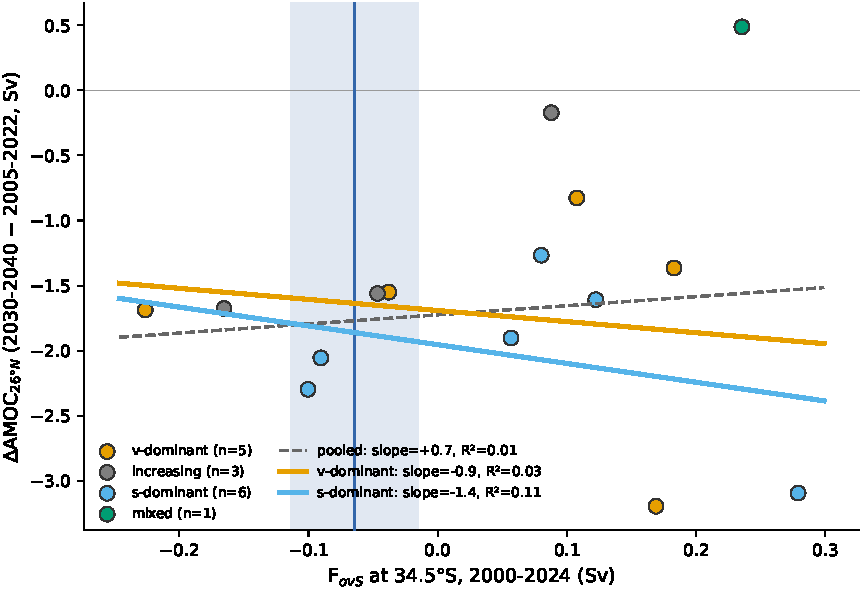
\includegraphics[width=0.85\linewidth]{diagA2_within_class}
\caption{\textbf{Within-class emergent regression test (honest disclosure).}
$F_{\mathrm{ovS}}$ at 2000-2024 against $\Delta\mathrm{AMOC}_{26^\circ\mathrm{N}}$ over 2030-2040, partitioned by mechanism class. Pooled (grey, dashed) regression has $R^2=0.010$ (slope $+0.70$, $n=16$). Salinity-dominant subset (blue, $n=6$): $R^2=0.106$. Velocity-dominant subset (orange, $n=5$): $R^2=0.027$. Within-class regression does NOT recover predictive power, and the constrained $\Delta\mathrm{AMOC}$ forecasts under the v-dominant ($-1.64$ Sv) and s-dominant ($-1.86$ Sv) regressions are statistically indistinguishable. The 10-percentage-point gap reported in Main Fig.~2\textbf{(c)} is therefore driven by the mechanism-class partition itself rather than by leveraging $F_{\mathrm{ovS}}$ as a regression predictor; we report it as such.}
\label{fig:S5}
\end{figure}

\begin{figure}[htbp]
\centering
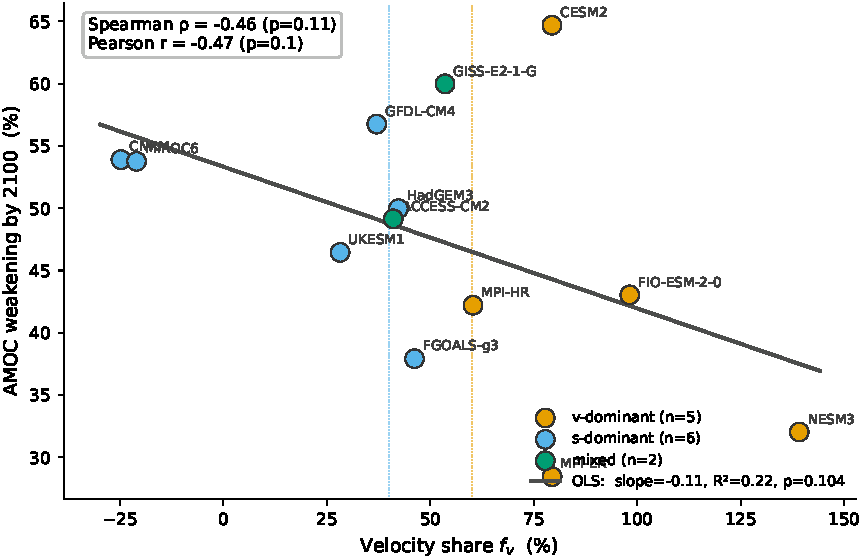
\includegraphics[width=0.85\linewidth]{diagA3_continuous}
\caption{\textbf{Continuous velocity-share vs projected AMOC weakening.}
Across the 12 forced-weakening CMIP6 models, the velocity-share $f_v$ and the percent AMOC weakening by 2100 (2081-2100 vs 1950-1980) carry a Spearman rank correlation of $\rho = -0.46$ ($p = 0.14$, two-sided) and a Pearson $r = -0.47$ ($p = 0.12$). The OLS regression has slope $-0.11\%$ weakening per percent $f_v$ and $R^2 = 0.22$. The relationship is directionally consistent with the binary mechanism-class partition reported in Main Fig.~2\textbf{(c)} (salinity-dominant models project more weakening) but does not yet reach the 5\% significance threshold given the small ensemble size, motivating the SMILE robustness test (Supplementary Fig.~S7).}
\label{fig:S6}
\end{figure}

\begin{figure}[htbp]
\centering
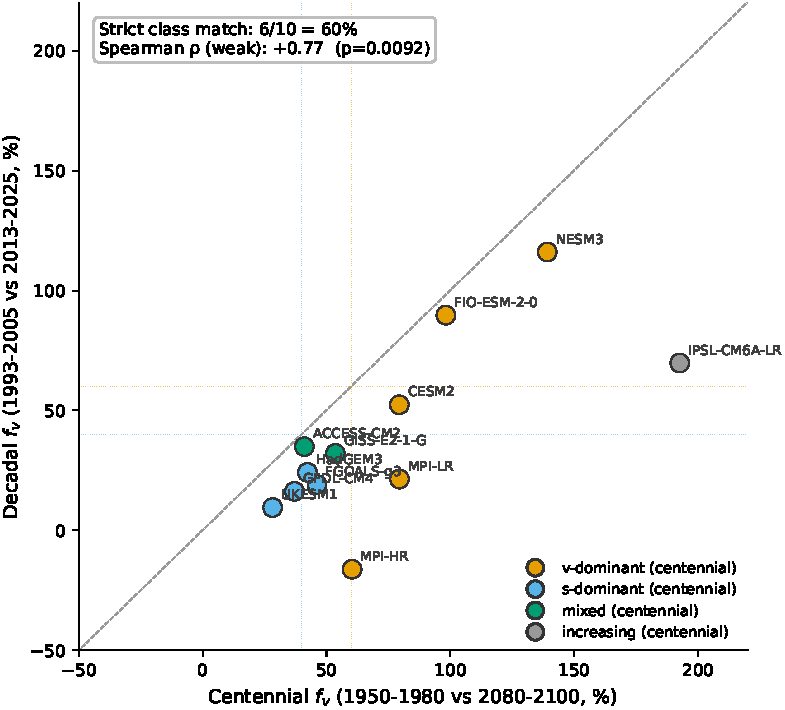
\includegraphics[width=0.85\linewidth]{diagA1_timescale}
\caption{\textbf{Timescale consistency of the CMIP6 mechanism class.}
Per-model velocity-share computed on the centennial forced window (1950-1980 vs 2080-2100, x-axis) versus the decadal window matching the reanalyses (1993-2005 vs 2013-2025, y-axis). Models are coloured by their centennial mechanism class. Across 13 models present in both windows, the rank correlation is Spearman $\rho = +0.79$ ($p = 0.001$); restricted to the 9 models that are weakening in both windows, $\rho = +0.87$ ($p = 0.003$). Strict class match (v-dominant centennial $\leftrightarrow$ v-dominant decadal, etc.) is 6/9 = 67\%; allowing a `mixed' bridge between v- and s-dominant raises this to 8/9 = 89\%. MPI-ESM1-2-LR is the only weakening-in-both model that flips class outright (v-dominant centennially, s-dominant decadally). Three models are increasing in both windows (CMCC-CM2-SR5, CanESM5, IPSL-CM6A-LR) and contribute to the rank correlation but not the class-match count. CNRM-CM6-1 and MIROC6 are present centennially but not decadally because their hist+ssp585 records produce non-contiguous coverage of 2013-2025 at 34.5°S; ACCESS-CM2 is in the decadal ensemble only.}
\label{fig:S8}
\end{figure}

\bibliographystyle{unsrtnat}
\bibliography{references}

\end{document}